%Incidencia de una onda plana a 45° con n_i = 1, n_t = 1.46   

\documentclass[tikz,border=1cm]{standalone}

\usepackage{tikz}
\usetikzlibrary{decorations.pathreplacing,decorations.pathmorphing}

\begin{document}


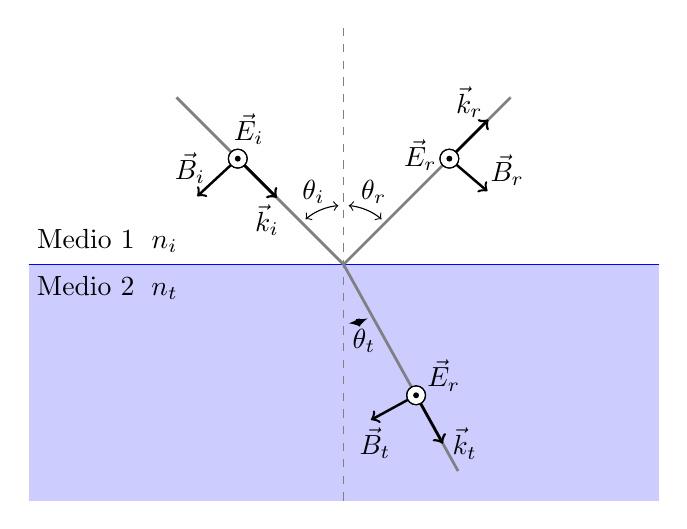
\begin{tikzpicture}%[   ESTO PONE LAS RAYAS QUE USO EN EPSEJOS
%    interface/.style={
        % The border decoration is a path replacing decorator. 
        % For the interface style we want to draw the original path.
        % The postaction option is therefore used to ensure that the
        % border decoration is drawn *after* the original path.
%        postaction={draw,decorate,decoration={border,angle=-45,
%                    amplitude=0.3cm,segment length=2mm}}},
%    ]



%-------------------------------------------- Incidence media
\fill[blue!20] (-4,-3) rectangle (4,0);
% Interface
\draw[blue,line width=.5pt](-4,0)--(4,0); %%..5pt, interface]
% Vertical dashed line
\draw[dashed,gray,](0,-3)--(0,3);
% Media names
\node at (-3,.3) {Medio 1 $\; n_i$}; 
\node at (-3,-.3) {Medio 2 $\; n_t$};

%--------------------------------------------  Incident Wave
\draw[gray, line width=1pt](0:0cm)--(135:3cm);  % Light trajectory
\path (0,0)++(112.5:1cm)node{$\theta_i$};       % Angle
\draw[<->](95:.75cm)arc(95:130:.75cm);
 
    \draw[->,line width=1pt](135:1.9cm)--(135:1.2cm);    %Wave vector
    \path (0,0)++(141:0.9cm)node[left]{$\vec{k}_i$};     %Wave vector label
    
    \draw[->,line width=.9pt](135:1.9cm)--(155:2.05cm);  %B vector
    \path (0,0)++(148:2.3cm)node{$\vec{B}_i$}; 
    
    \path (0,0)++(125:2.1cm)node{$\vec{E}_i$};       % E vector
    
    \draw [fill= white](135:1.9cm)circle (0.12cm); % Vector perp. to surface
    \draw [black](135:1.9cm)circle (0.12cm);
    \filldraw[fill=black](135:1.9cm) circle(0.03cm); %%
    
%--------------------------------------------  Reflected Wave
\draw[gray,line width=1pt](0:0cm)--(45:3cm);  % Light trajectory
\path (0,0)++(67.5:1cm)node{$\theta_r$};       % Angle
\draw[<->](85:.75cm)arc(85:50:.75cm);
 
    \draw[->,line width=1pt](45:1.9cm)--(45:2.6cm);    %Wave vector
    \path (0,0)++(47.5:2.8cm)node[left]{$\vec{k}_r$};     %Wave vector label
    
    \draw[->,line width=.9pt](45:1.9cm)--(27:2.05cm);  %B vector
    \path (0,0)++(30:2.4cm)node{$\vec{B}_r$}; 
    
    \path (0,0)++(55:1.7cm)node{$\vec{E}_r$};       % E vector
    
    \draw [fill= white](45:1.9cm)circle (0.12cm); % Vector perp. to surface
    \draw [black](45:1.9cm)circle (0.12cm);
    \filldraw[fill=black](45:1.9cm) circle(0.03cm); %%

%--------------------------------------------  Transmitted Wave
\draw[gray,line width=1pt](0:0cm)--(-61:3cm);  % Light trajectory
\path (0,0)++(-75:1cm)node{$\theta_t$};       % Angle
\draw[latex - latex](-85:0.75cm)arc(-85:-66:.75cm);
 
    \draw[->,line width=1pt](-61:1.9cm)--(-61:2.6cm);    %Wave vector
    \path (0,0)++(-61:2.6cm)node[right]{$\vec{k}_t$};     %Wave vector label

    \draw[->,line width=.9pt](-61:1.9cm)--(-80:2.005cm);  %B vector
    \path (0,0)++(-80:2.3cm)node{$\vec{B}_t$}; 
    
    \path (0,0)++(-48:1.9cm)node{$\vec{E}_r$};       % E vector
    
    \draw [fill= white](-61:1.9cm)circle (0.12cm); % Vector perp. to surface
    \draw [black](-61:1.9cm)circle (0.12cm);
    \filldraw[fill=black](-61:1.9cm) circle(0.03cm); %%     
 


\end{tikzpicture}


\end{document}